\documentclass{beamer}
%\usepackage[ngerman]{babel}              
%\usepackage[applemac]{inputenc}
\usepackage{multimedia} 

\setbeamertemplate{navigation symbols}{}
\mode<presentation>{
\usetheme{Warsaw} \setbeamercovered{transparent}
}

\title[]{Calibration of a Kinect-Projector System}
\author[Nikolas Engelhard]{\texorpdfstring {\underline{Nikolas Engelhard} \\ Supervisor: Dr. Juergen Sturm}
{Autor}
}
\institute{CVPR\\ Prof. Dr. Cremers}
\date{\today}

%\titlegraphic{
%\begin{minipage}{0.45\textwidth}
%\centerline{\includegraphics[width=.75\textwidth]{some_logo}}
%\end{minipage}
%}


\begin{document}

\frame{\titlepage}

%\section*{Overview}
%\frame{\tableofcontents}

\section{Problem}
\frame{
%\frametitle{first title}
%\begin{center}
Undistort the projector's image

\begin{figure}[t]
\centering
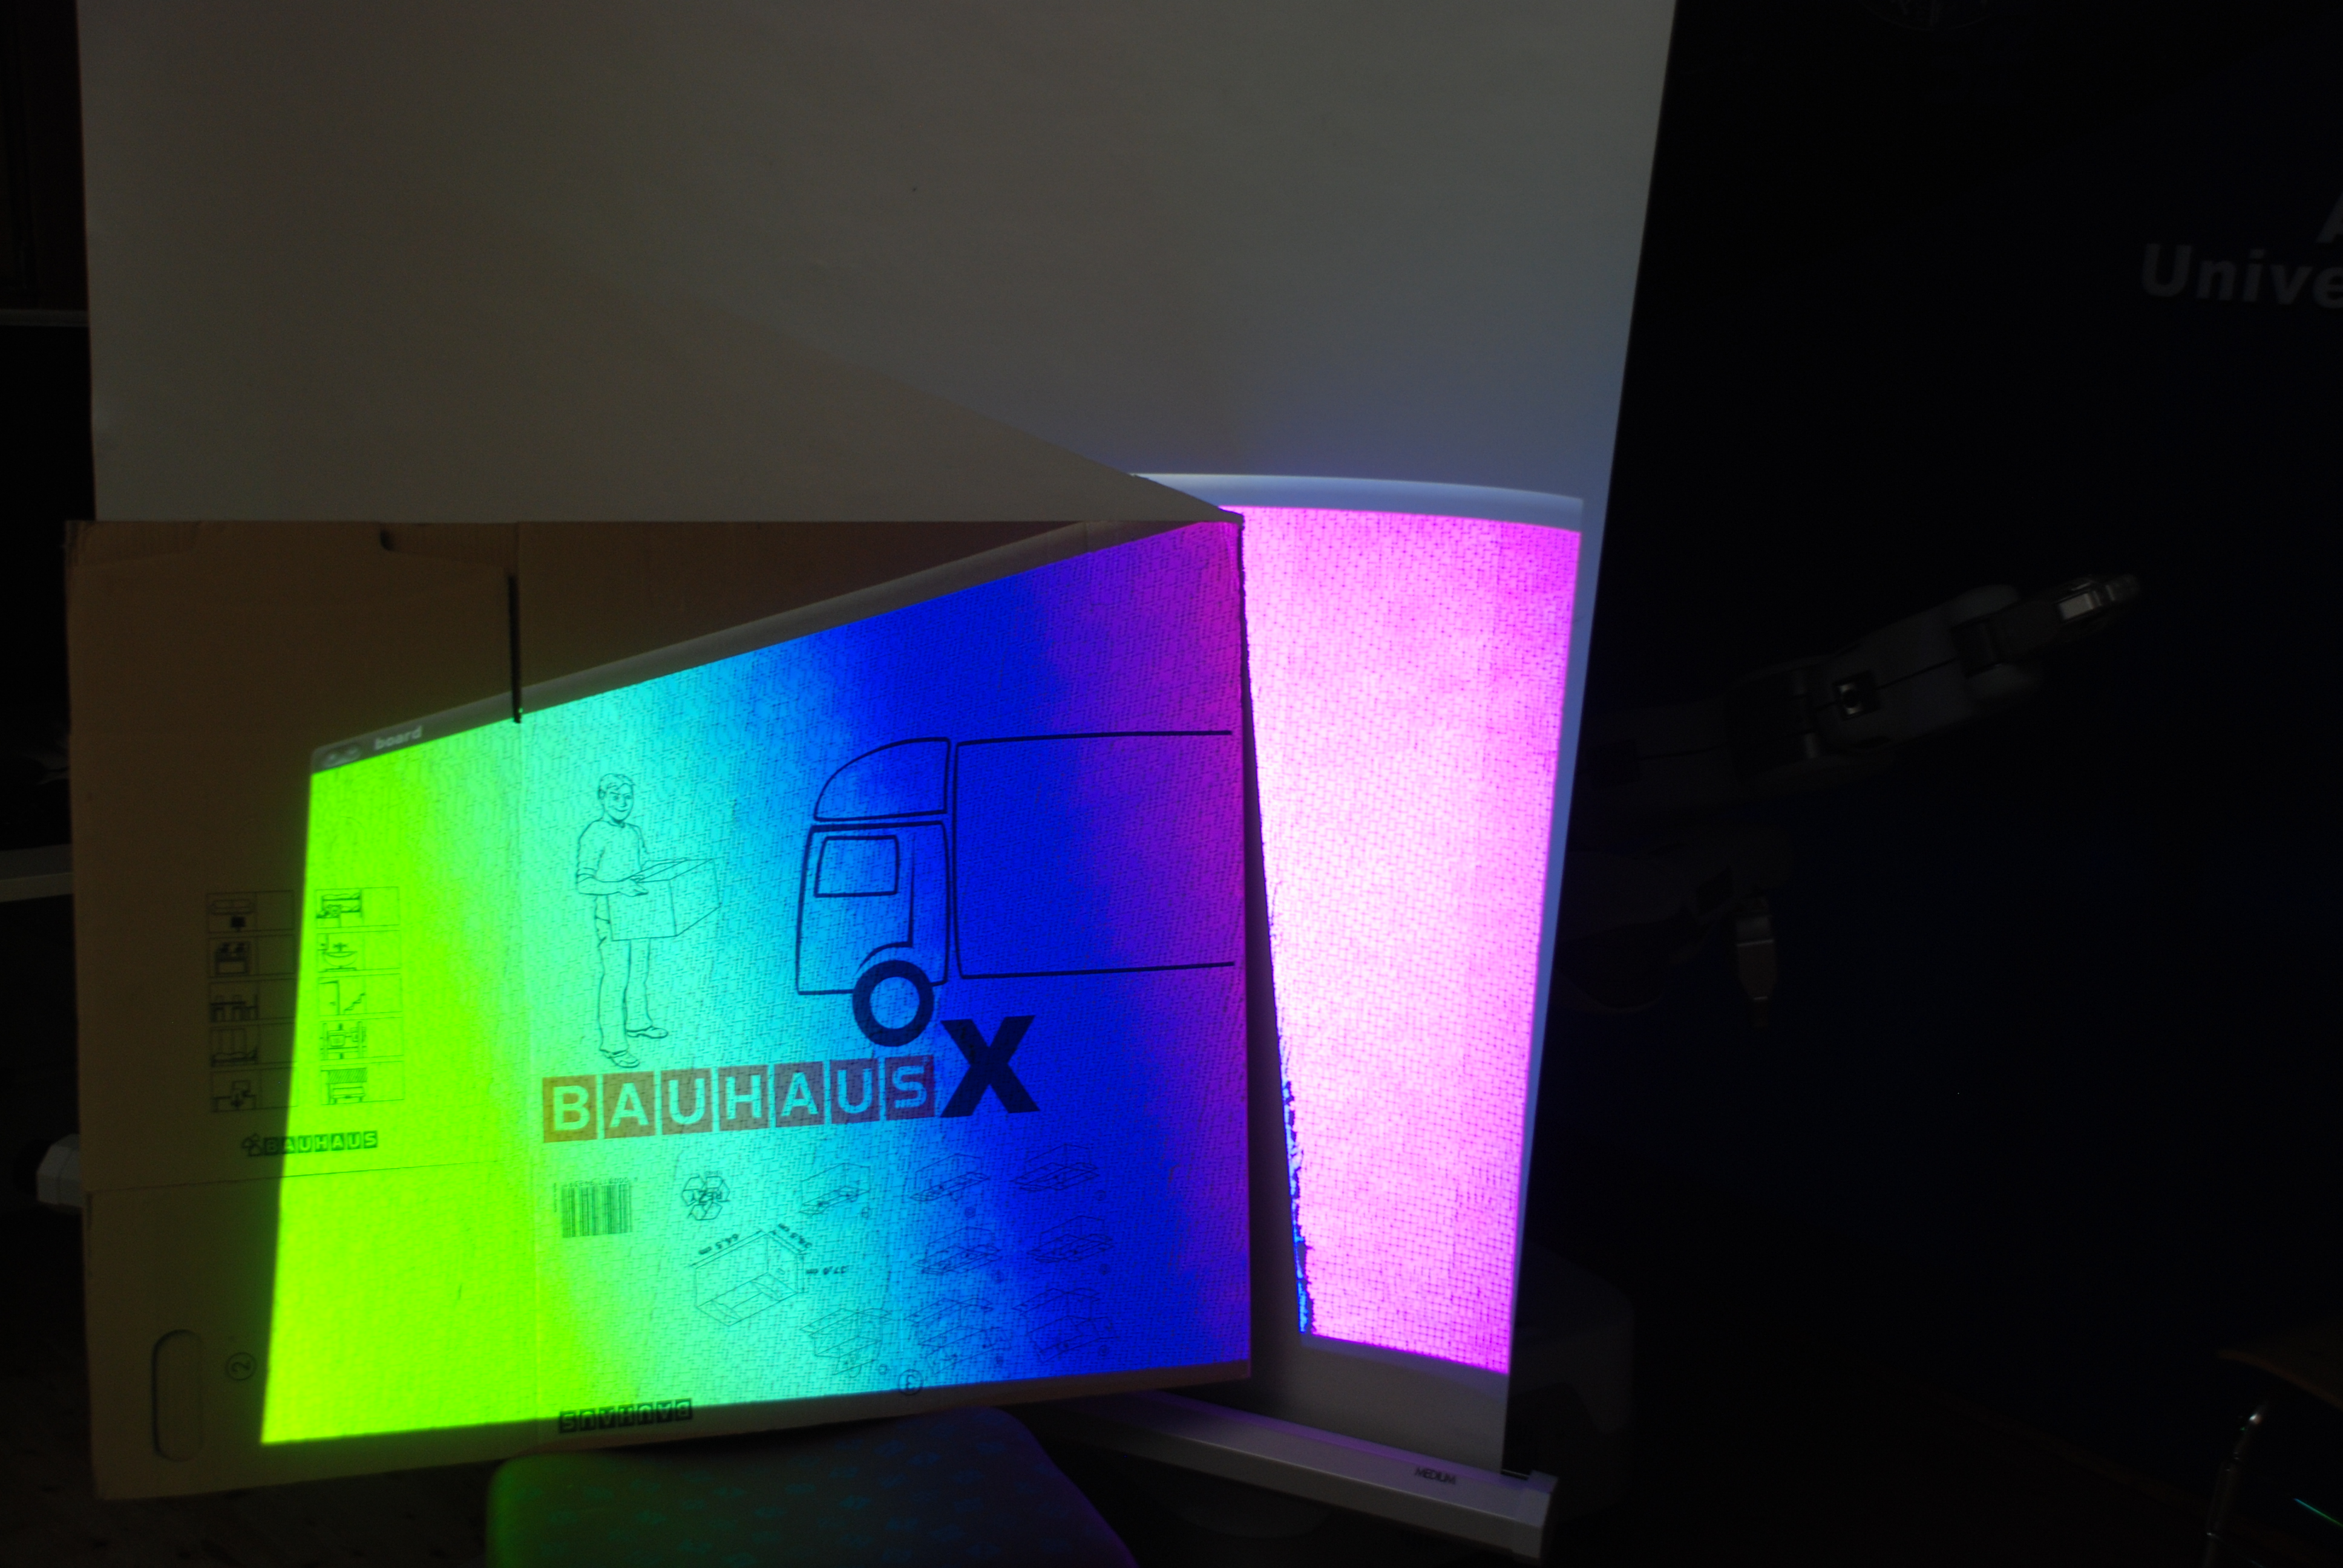
\includegraphics[height=4cm]{img/img_1.JPG}
\caption{Distortion due to projective transformation}
\end{figure}

%\end{center}

%\begin{itemize}
%\item Mapping: \\ Which features should be remembered?
%\item Localisation: \\ Which features are to be expected?
%\item Navigation: \\  Which obstacles can vanish?
%\end{itemize}


}

\section{Approach}

\frame{
\frametitle{Approach}

\begin{itemize}
\item Projection of a known pattern (checkerboard) onto the wall
\item Recognition of feature points in the Kinect-image and extraction of their 3d-pose
\item Computation of homography between wall and projector's image plane
\item Computation of the projector's projection matrix
\end{itemize}


%\begin{figure}[t]
%\centering
%\includegraphics[height=4cm]{grey.pdf}
%\caption{Moving objects are highlighted}
%\end{figure}
}



\frame
{
  \frametitle{Definition of the wall's coordinate system}
		
  \begin{itemize}
  \item Projection of a checkerboard pattern onto the wall
  \item 3d position of pattern's center point is used as origin 
  \item a plane is fitted to all 3d points within the pattern region and used as $z=0$-plane 
  \item Rotation around plane-normal is last free parameter
  	\begin{itemize}
  	\item usage of Kinect's IMU (y-axis parallel to $\vec{g}$)
  	\end{itemize}
  \item no assumption on the relative or absolute pose of projector or camera
  \end{itemize}
}

\frame
{
\frametitle{Homography}
\begin{itemize}
\item Extraction of all checkerboard corners in a single image
\item Extraction of 3D position of all points and transformation in the wall-frame
\item set of 3d-2d Correspondences:
 $\left(\begin{array}{c}x \\y \\1\end{array}\right) = P \left(\begin{array}{c}X\\Y \\Z \\1\end{array}\right) $
 \item All 3d-points are on the $z=0$-plane: 
 $\left(\begin{array}{c}x \\y \\1\end{array}\right) = H \left(\begin{array}{c}X \\Y \\1\end{array}\right) $
\end{itemize}
}

\frame
{
\begin{itemize}
\item each pair generates a constraint of the form $x_i \times HX_i = 0 $
\item this leads to three equations, which are linearly dependend
\end{itemize}
%{ \tiny
%$ { \underbrace{\left(\begin{array}{cccccccccccc}0 & 0 & 0 & 0 & -X_i & -Y_i & -Z_i & 1 & y_iX_i & y_iY_i & y_iZ_i & y_i \\X_i & Y_i & Z_i & 1 & 0 & 0 & 0 & 0 & -x_iX_i & -x_iY_i & -x_iZ_i & -x_i \\ & & & & & & \ldots \\ & & & & & & \ldots \end{array}\right) }_{A \in M(2i \times 12,\mathbb{R}) } \left(\begin{array}{c}P_{11} \\ P_{11} \\P_{12} \\P_{13} \\P_{14} \\P_{21} \\P_{22} \\P_{23} \\P_{24} \\P_{31} \\P_{32} \\P_{33} \\ P_{34}  \end{array}\right)  = 0} 	$ }
{ \tiny
$ { \underbrace{\left(\begin{array}{ccccccccc}0 & 0 & 0 &  -X_i & -Y_i & 1 & y_iX_i & y_iY_i & y_i \\X_i & Y_i & 1 & 0 & 0  & 0 & -x_iX_i & -x_iY_i & -x_i \\ & & & & &  \ldots \\ & & & & & \ldots \end{array}\right) }_{A \in M(2i \times p,\mathbb{R}) } \left(\begin{array}{c}H_{11} \\ H_{11} \\H_{12} \\H_{13}  \\H_{21} \\H_{22} \\H_{23} \\H_{31} \\H_{32} \\H_{33}  \end{array}\right)  = 0} 	$ }


\begin{itemize}
\item Optimizing $A H = 0$ leads to trivial solution $h=0$
\item P only defined up to scale $\Rightarrow$ new constraint $||h|| = 1$
\item solvable via SVD and cv::getHomography
\end{itemize}

}

\frame 
{
\frametitle{Normalization}
\begin{itemize}
\item 3d coordinates are given in meter 
\item pixel coordinates are much larger
\item Compute normalizing transformations $T_{3d}$, and $T_{2d}$ so that both sets are zero-centered and have a mean norm of $\sqrt{2}$
\item TODO: eval of reprojection error
\end{itemize}
}

\section{Undistortion of an image}
\frame{
\frametitle{Finding the optimal projection area}
\begin{itemize}
\item Find the largest axis aligned rectangle with the side ratio of the projected image
\end{itemize}

TODO: images
}

\frame{
\frametitle{Undistort the image}
\begin{itemize}
\item goal: Find
\end{itemize}

}


\end{document} 